%!TEX root = ../../thesis.tex
%*******************************************************************************
%****************************** Background Chapter *********************************
%*******************************************************************************

\chapter{Foundations}
\label{chap:foundations}
\ifpdf
    \graphicspath{{Chapters/Background/Figs/}{Chapters/Background/Figs/}{Chapters/Background/Figs/}}
\else
    \graphicspath{{Chapters/Background/Figs/}{Chapters/Background/Figs/}}
\fi
In the previous chapter, we defined the problems for software development and presented an overview of our solution.
Consequently, this chapter is built upon the existing knowledge and theories developed in the field of Software Engineering.
This chapter provides an overview of the relevant literature and identifies the key concepts and theories necessary for the research. 
Firstly, we discuss \textit{\ac{ui} Prototyping} (see section \ref{background:section:uiprototyping}) explaining the creation of a \ac{ui} simulation and testing for refining the design ideas and user requirements.
Then, we explain \textit{Low/No-code methods} (see section \ref{background:section:lowcode}) and citizen development of the software products. 
Then we describe the \textit{\ac{mbse}} approaches and meta-models (see section \ref{background:section:mbse}).
We clarify \textit{Task-Based Usability Testing} (see section \ref{background:section:task}) for reviewing and refining the product. 
Later we define the concept of \textit{\ac{ui} Experimentation} (see section \ref{background:section:experimentproduct}) and \textit{A/B testing}. 
Finally, we explain the \textit{LEAN software development process} (see section \ref{background:section:lean}), explaining the \textit{Build, Measure} and \textit{Learn} phases.

% To build the foundation of our approach, we present UI Prototyping (see section \ref{background:section:uiprototyping}), Low and No code (see section \ref{background:section:lowcode}), Model-Based Software Engineering (MBSE) (see section ), Task-Based Usability Testing (see section \ref{background:section:task}), and Experimental Product Design (see section \ref{background:section:experimentproduct}) and derive some Design Requirements (see section \ref{background:section:designReqs}).
%********************************** % Crowdsourcing of Software Products **************************************
% \section{Crowdsourcing of Software Products}
% \label{background:section:crowdsourcing}
% ***************************** \textbf{Optional section} ***************************** \\\\
% Iterative feedback from potential customers can help improve the development of software products \cite{article:lean:eric}.
% To do that, we can use crowdsourcing.
% Crowdsourcing refers to outsourcing value-creating activities from a company by an open call to a large, undefined group of users to get feedback \cite{article:crowdsourcing:leimeister}.
% The word crowdsourcing is a combination of crowd and outsourcing.
% Crowdsourcing often involves less specialized and more generalized groups of participants than outsourcing \cite{article:crowdsourcing:estelles}.
% Some advantages of crowdsourcing include lowered costs, improved speed, quality, flexibility, and scalability \cite{article:crowdsourcing:prpic}.
% Researchers have used crowdsourcing in many research approaches, including \textit{crowd testing, crowd funding, crowd ideation, crowd logistic, crowd production, crowd promotion,} and \textit{crowd support} over the last few years \cite{article:crowdsourcing:durward}.
% In our approach to finding a solution, we focus more on crowd-testing and crowd-ideation.

% \paragraph{Crowd Testing:}
% The companies use crowd-testing to evaluate different running software products with the users.
% A growing trend in software testing is crowd testing, which utilizes the benefits, effectiveness, and efficiency of crowdsourcing and cloud platforms \cite{article:crowdsourcing:latoza}.
% Crowd testing is considered when the software is more user-centric: i.e., software with a broad user base whose success is evaluated by user input.
% CrowdStudy \cite{article:crowdsourcing:nebeling} is a method that enables developers to assess the usability of their web interfaces using crowd workers from Amazon Mechanical Turk\footnote{Amazon Mechanical Turk: \url{https://www.mturk.com}}.
% CrowdCrit \cite{article:crowdsourcing:luther} is another tool that uses Amazon Mechanical Turk to support designers in validating created posters in the form of uploaded images.
% Similarly, \textit{Interactive event-flow graphs} and \textit{GUI-level (Graphical User Interface) guidance} \cite{article:crowdsourcing:chen} are the two techniques to increase crowd testers' coverage for GUI using crowd-testing.

% \paragraph{Crowd Ideation:}
% Design can be infused with creativity by online crowds, but using traditional strategies to harness them, such as large-scale ideation platforms, requires organization and time \cite{article:crowdsourcing:andolina}.
% Hence, crowd ideation is used to build new and improved versions of existing software product ideas with the consumers.
% Under manipulations of task complexity, idea representation, and procedural guidance, Shixuan Fu et al. \cite{article:crowdsourcing:fu} examine how cognitive load is altered during idea generation and convergence with crowds.
% ERICA \cite{article:crowdsourcing:erica} is a tool that uses expert knowledge to validate diverse crowd answers.
% Crowdboard \cite{article:crowdsourcing:andolina} is a tool used to engage crowds in real-time brainstorming, concept mapping, and other design processes at an early stage of the design process.
% There were, however, no approaches that directly addressed prototype application areas.
% \clearpage
%********************************** % UI Prototyping **************************************
\section{UI Prototyping}
\label{background:section:uiprototyping}

\ac{ui} prototyping is a valuable tool for designers, allowing them to quickly and easily test and refine \ac{ui} designs \cite{article:prototyping:gould}.
\ac{ui} prototyping creates a simplified \ac{ui} version to test and iterate on design ideas before building the final product.
It also helps gather feedback from users and stakeholders \cite{misc:prorotypes:lauff} and identify any usability issues before investing significant time and resources into the final product.
From paper to \ac{html} code, everything could be a prototype, including various techniques like \texttt{Paper Prototypes}\footnote{\textbf{Paper prototyping:} It is a method of creating a preliminary version of a \ac{ui} using paper and pen.}, \texttt{Wireframes}\footnote{\textbf{Wireframe:} A wireframe is an essential visual representation of the layout and structure of a product, showing the placement of text, images, and buttons.}, \texttt{Mockups}\footnote{\textbf{Mockup:} A mockup is a more detailed version of a wireframe, typically created in color and with more realistic graphics and images.}, and \texttt{Interactive Prototypes}\footnote{\textbf{Interactive Prototype:} An interactive prototype is a fully functional representation of a product, design, or feature.}.
Moreover, \ac{ui} Prototypes can be classified as \textit{High-Fidelity} and \textit{Low-Fidelity} prototypes.
The comparison by Jim Rudd et al. \cite{article:prototyping:highlowfidelity} on high and low-fidelity prototyping, based on its advantages and disadvantages, is explained further.

\paragraph*{Low-Fidelity Prototypes:}
\textit{Low-fidelity} prototypes (see figure \ref{fig:background:lowfidelity}) usually have limited functions and little interaction prototyping effort. 
They mainly focus on explaining concepts, design alternatives, and screen layouts. 
Storyboard presentations, cards, proof-of-concept prototypes, paper prototypes, etc., come under this category.
For instance, paper-based prototypes are simple, low-fidelity mockups that can be quickly and cheaply created using paper and pencil (see figure \ref{fig:background:paperPrototyping}).
In this case, the \ac{ui} designers use simple text, lines, and forms to hand-draw concepts. 
Instead of aesthetics, the focus is on speed and creative ideas.
To simulate user flows (as shown in figure \ref{fig:background:paperprototypes}), designers lay paper screens on the floor, table, or pinned to a board.
Therefore, these prototypes emphasize communicating, educating, and informing rather than training, testing, and codification \cite{misc:prototyping:low}.
The advantages of low-fidelity prototypes are rapid development, lower development cost, addressing issues, and usefulness for a proof-of-concept \cite{article:prototyping:highlowfidelity}.
Similarly, the disadvantages include limited error checking, difficulty with usability testing, navigation, flow limitation, etc.
\begin{figure}[htbp!]
  \begin{subfigure}[b]{0.5\textwidth}
    \centering
    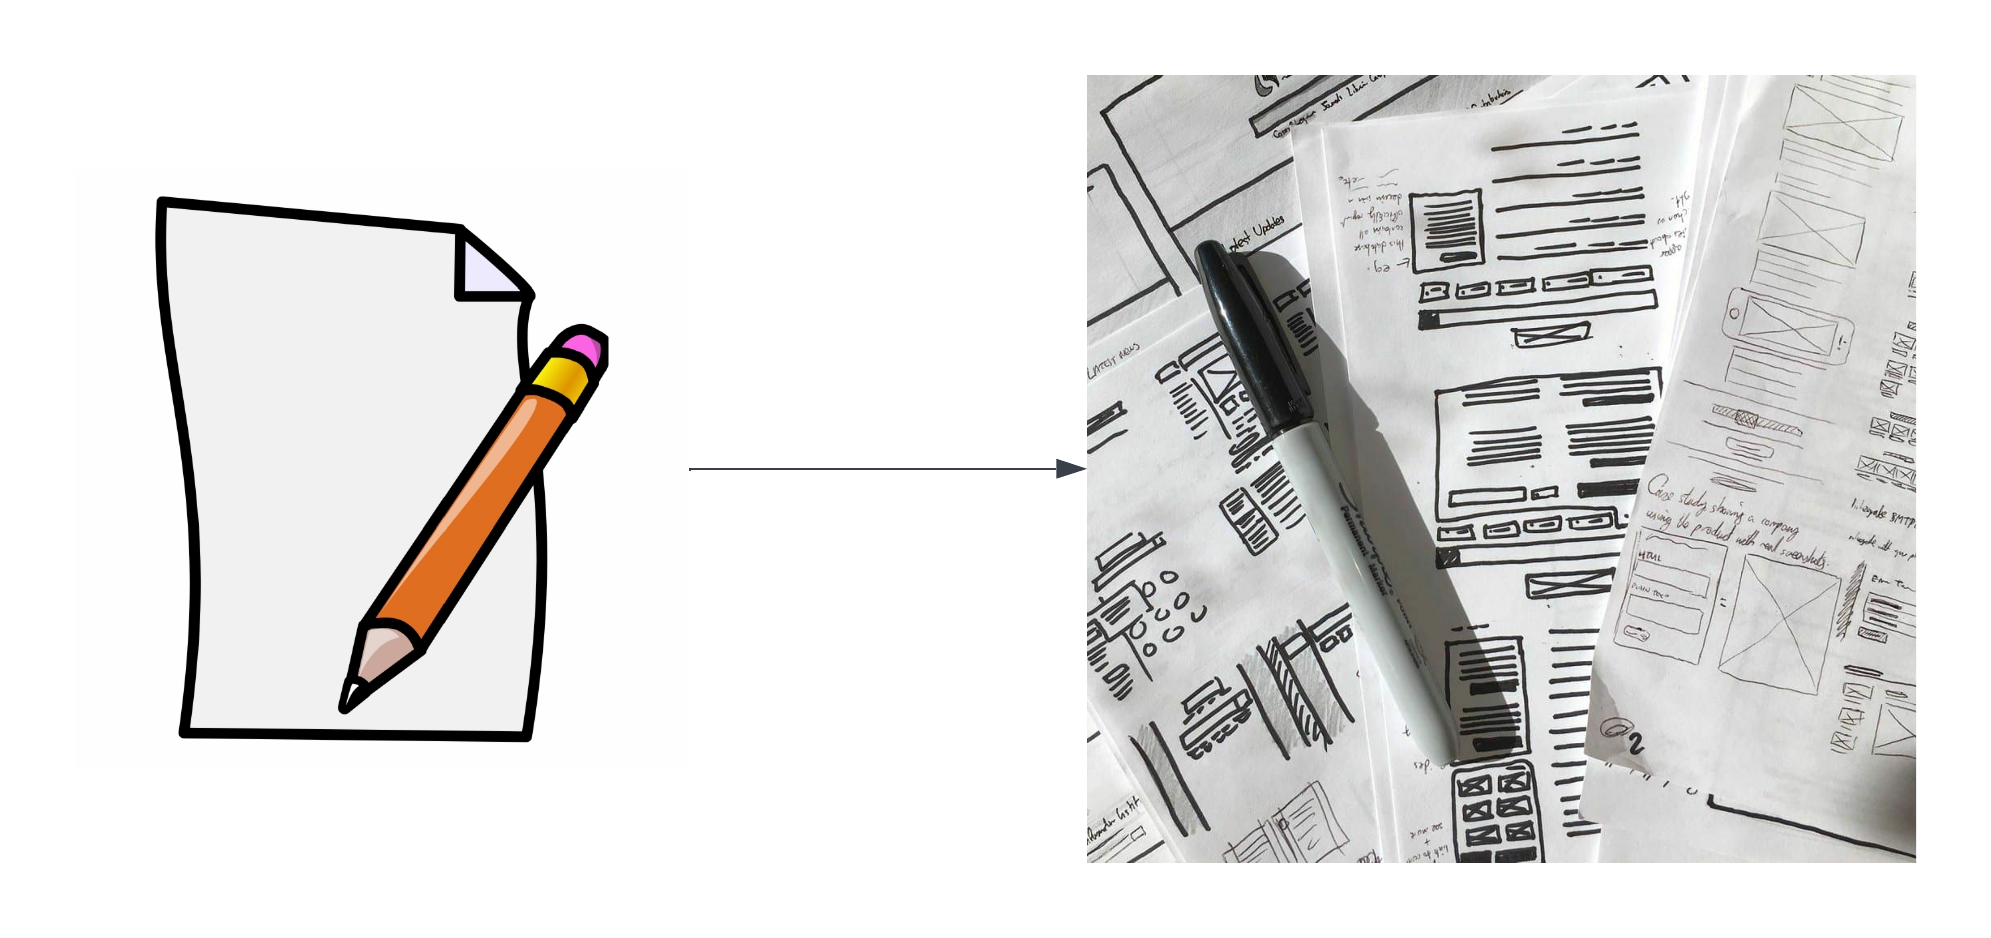
\includegraphics[width=\textwidth]{paperprototyping.png}
    \caption{Sketches and Whiteboard for Prototyping}
    \label{fig:background:paperPrototyping}   
  \end{subfigure}             
  \begin{subfigure}[b]{0.5\textwidth}
    \centering
    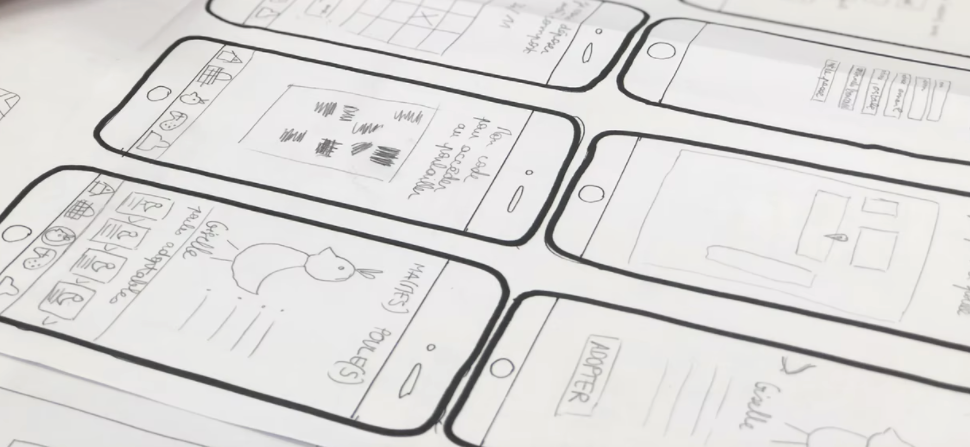
\includegraphics[width=\textwidth]{paperstepsprototypes.png}
    \caption[Paper-Based Prototypes]{Example on How the Paper-Based Prototypes Are Developed  \cite{misc:prototyping:uxpin}}
    \label{fig:background:paperprototypes}
  \end{subfigure}             
  \caption[Low-Fidelity Prototyping]{Low-Fidelity Prototyping}
  \label{fig:background:lowfidelity}
\end{figure}
\paragraph*{High-Fidelity Prototypes:}
Contrary to low-fidelity prototypes, \textit{high-fidelity} prototypes (see figure \ref{fig:background:uiPrototyping}) have full functionality and focus on the logical flow between screens and the user models of the system \cite{article:prototyping:exploratory}.
These prototypes are detailed, interactive mockups of a \ac{ui} designed to mimic the look and feel of the final product closely.
High-fidelity prototypes are often created using interactive prototyping tools, which allow designers to create realistic, interactive mockups of \ac{ui} designs \cite{article:prototyping:weichbroth}. 
These tools typically include a library of \ac{ui} elements and templates and the ability to create interactive transitions and animations.
The users can operate these prototypes, and the developers can collect information from the users through measurements.
Some advantages of high-fidelity prototypes are that they are user-driven, used for navigation and tests, and can also serve as a marketing tool for attracting potential customers \cite{article:prototyping:highlowfidelity}.
Therefore, these prototypes are typically more realistic and interactive than those created using other tools but may require more time and resources to develop and maintain.
At the same time, high-fidelity prototypes allow designers and developers to test and refine complex \ac{ui} concepts and interactions, ensuring the final product is user-friendly and practical.
Overall, low-fidelity prototypes and high-fidelity prototypes are both valuable tools in the design process, and the choice between the two will depend on the specific needs and goals of the project.
\begin{figure}[htbp]
  \begin{subfigure}[b]{0.5\textwidth}
    \centering
    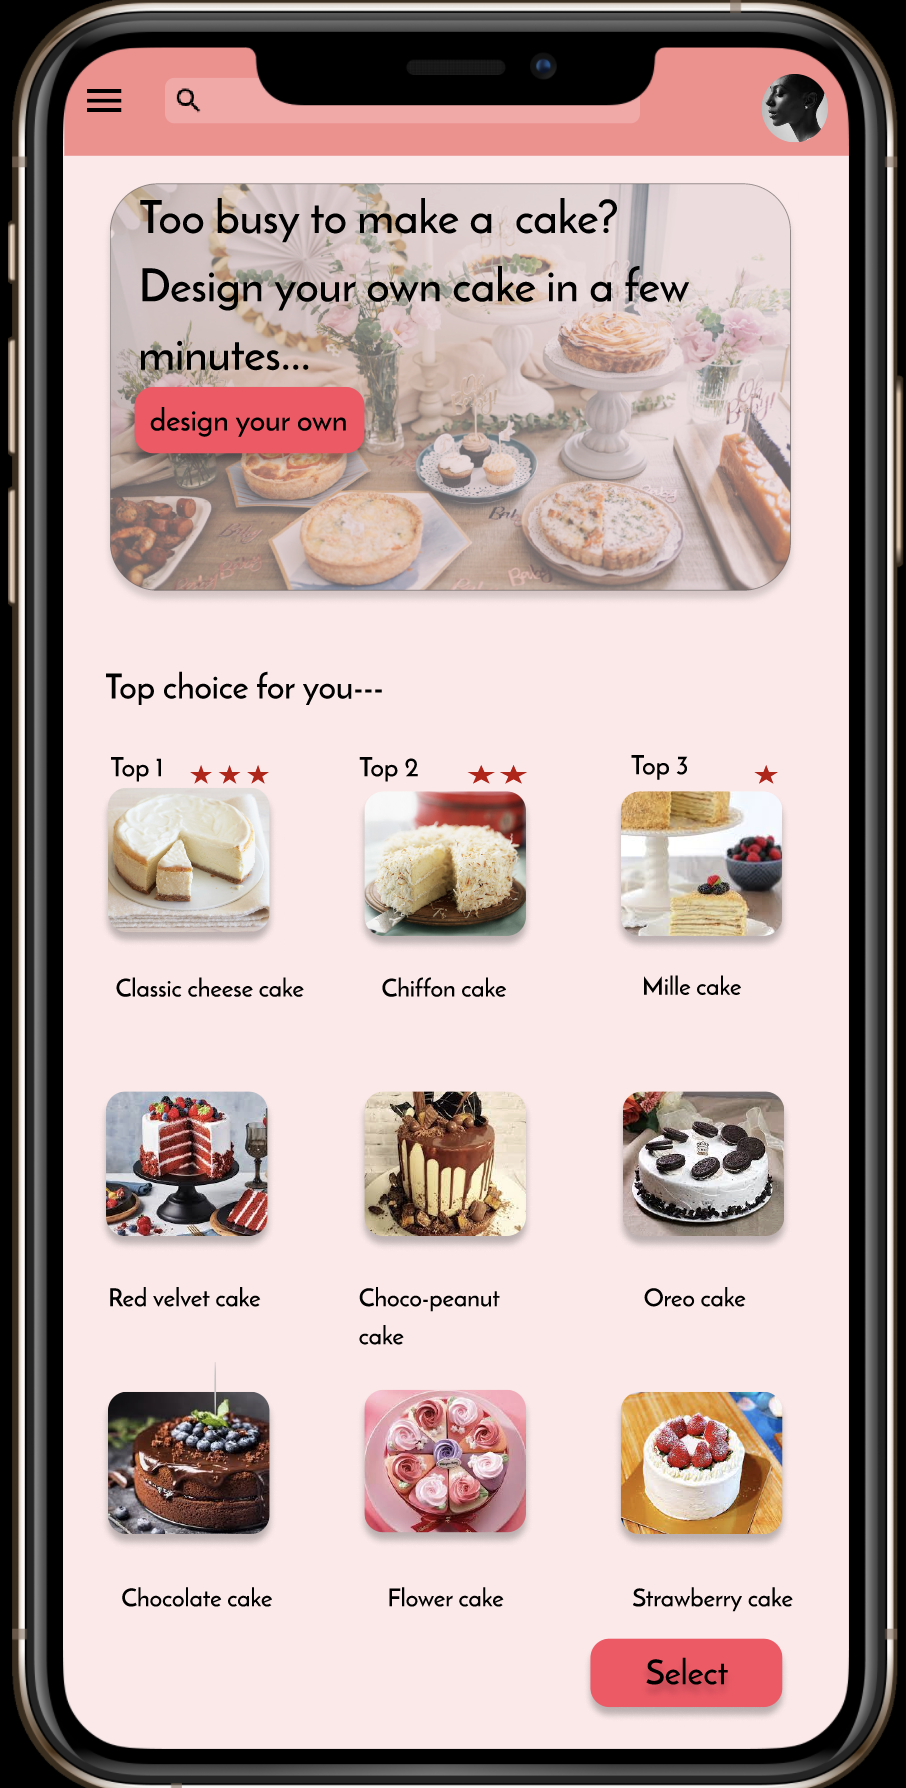
\includegraphics[width=0.5\textwidth]{high-fidelity-prototyping.png}
    \caption{Prototyping Page of a Cake Company}
    \label{fig:background:high1}   
  \end{subfigure}
  \begin{subfigure}[b]{0.5\textwidth}
    \centering
    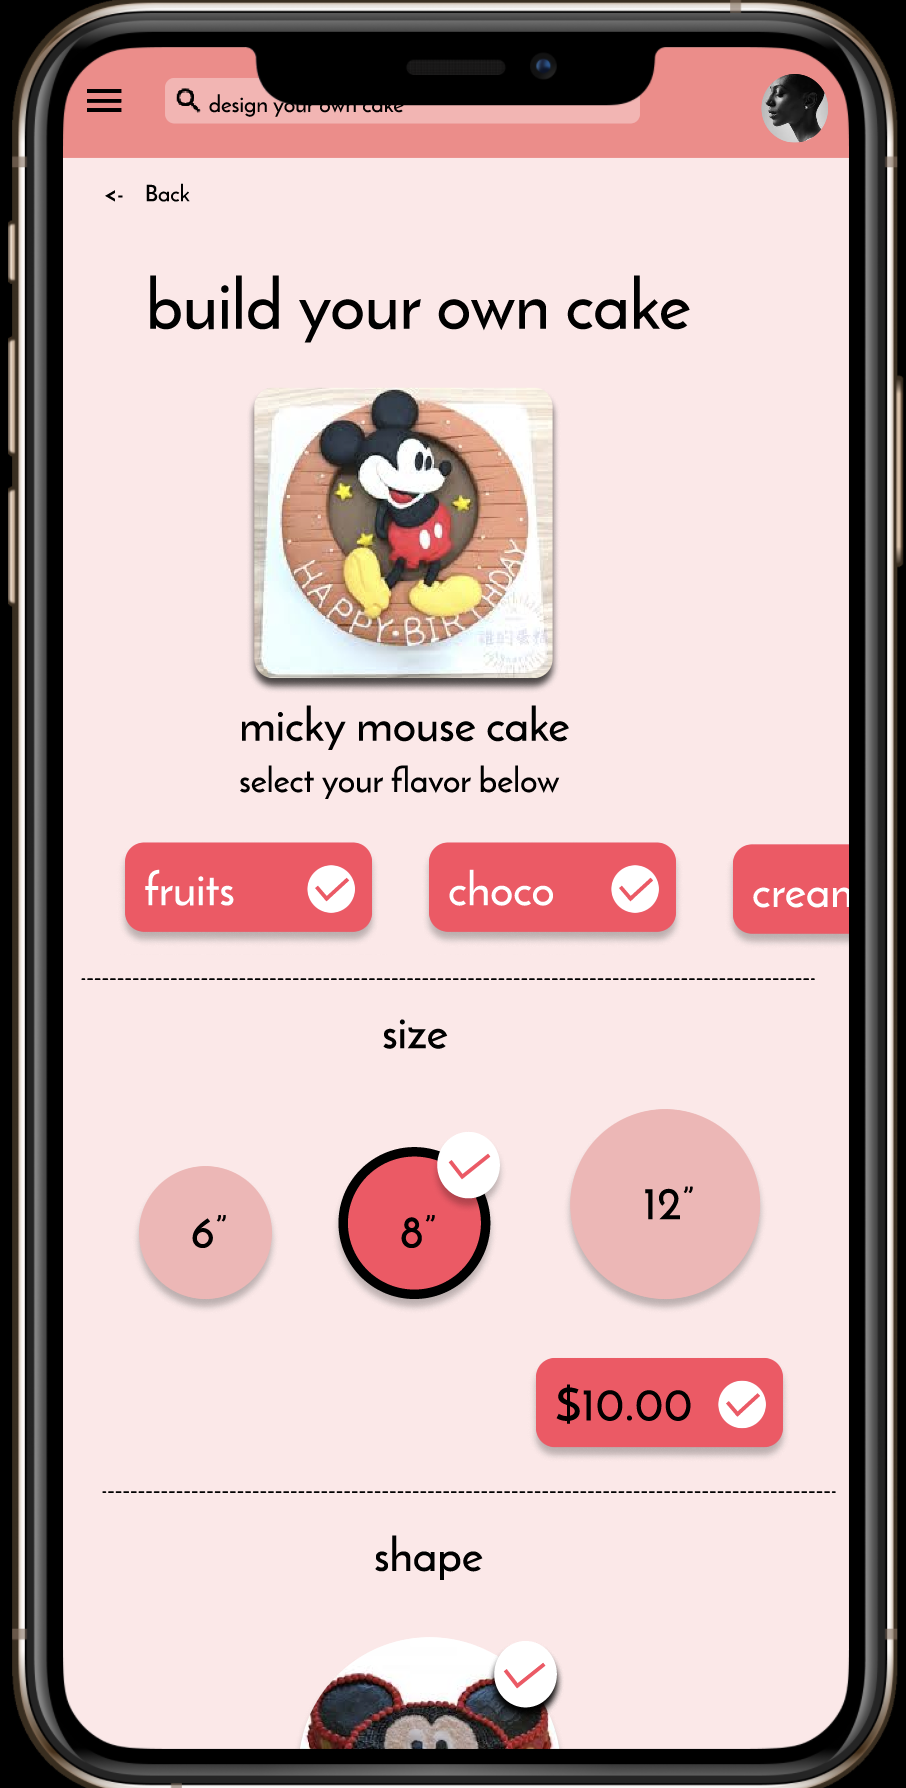
\includegraphics[width=0.5\textwidth]{high-fidelity-2.png}
    \caption{Prototyping Page to Customize a Cake}
    \label{fig:background:high2}   
  \end{subfigure} 
  \caption[High-Fidelity Prototyping]{High-Fidelity prototype: Model-Based UI Prototyping \cite{misc:prototyping:hfp}}
  \label{fig:background:uiPrototyping}
\end{figure}

UI prototyping has been an evaluation and testing technique according to \ac{ucd} methodology since the 1990s \cite{article:prototyping:preece}.
The evaluation of prototypes by users gives crucial feedback in iterative approaches for \ac{it} project management, especially agile methodologies \cite{article:prototyping:schwaber}.
Therefore, to build an exemplary \ac{ui}, a company can use this approach: develop a preliminary version of the \ac{ui}, test it with people, and make as many revisions as possible (without building the actual software) \cite{article:prototyping:gould}.
Figure \ref{fig:background:stepsPrototyping} shows a cycle representing the iterative development with prototypes.
The designers start the process by developing the \ac{ui} prototypes, which the stakeholders (e.g., customers and product managers) review. 
The \ac{ui} prototypes are refined from the feedback received, reiterating the cycle.
Therefore, designing \ac{ui} prototypes enables designers and stakeholders to communicate more effectively.
\begin{figure}[htbp!]
  \centering    
  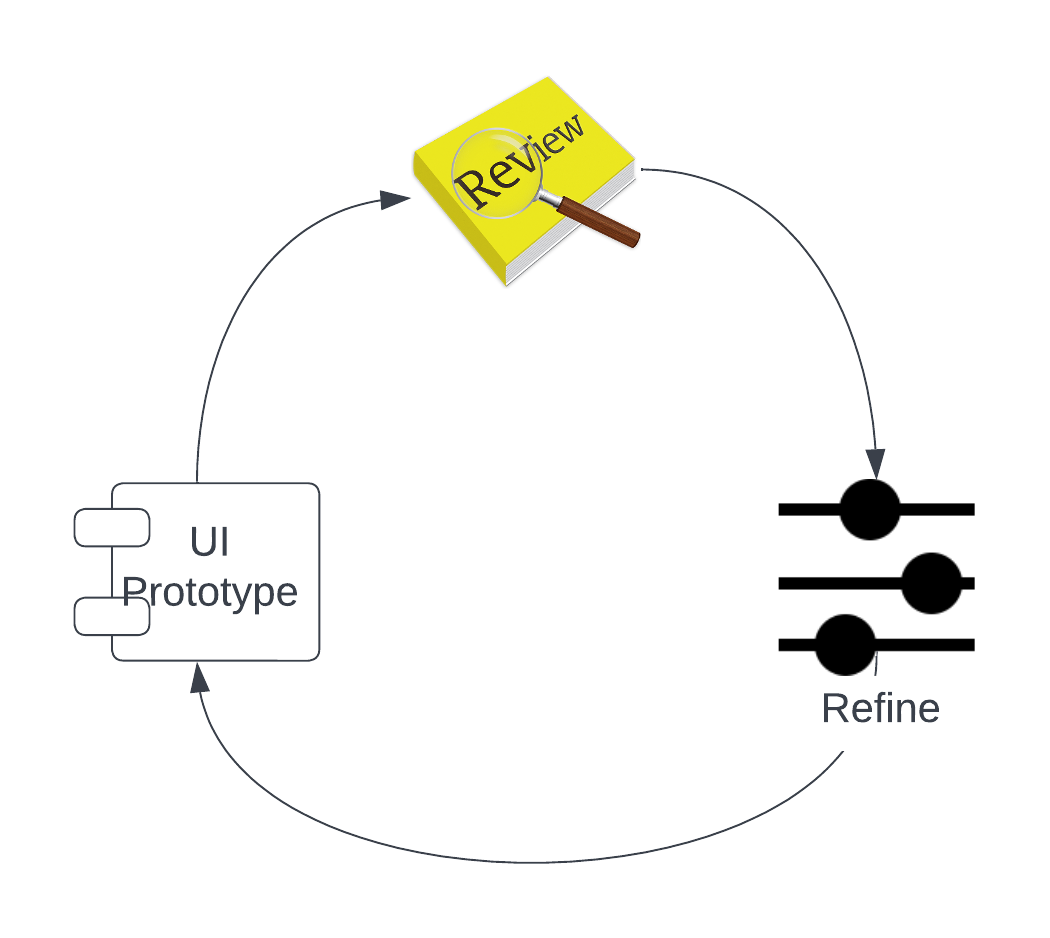
\includegraphics[width=0.6\textwidth]{PrototypingSteps.png}
  \caption[Steps of Prototyping]{Prototyping Steps for an Iterative Development}
  \label{fig:background:stepsPrototyping}
\end{figure}
Similarly, an interactive prototype helps visualize design concepts and communicate new requirements and expectations about a prospective system.
Iterative design requires multiple updates to the design's execution.

Since developing and updating the entire software system is complex and expensive, prototyping is a crucial step \cite{article:prototyping:szekely} in software development.
Simultaneously, prototypes might exclude many requirements, making the software more accessible, smaller, and less expensive to construct and change \cite{article:prototyping:szekely}. 
Thus, the main difference between a prototype and a software application is that in a prototype, the screens are designed images with no additional capabilities to display the design and flow. 
Moreover, usability testing to validate user requirements and prototype functionality is a part of the evaluation process for \ac{ui} prototypes \cite{article:prototyping:hoffnagle}.
Thus by using prototyping, there is usually more contact between the designers and users, resulting in fewer usability flaws and corrections at the end of development.
And finally, these mockups are then converted into actual UI elements in a software application, and a logical flow is established.

Overall, \ac{ui} prototyping is an essential part of the design process. 
It allows designers and developers to quickly test and refine \ac{ui} concepts, gather feedback from stakeholders and users, and identify any usability issues before investing significant time and resources into building the final product. 
Whether using low-fidelity prototypes to test basic layout and navigation concepts or high-fidelity prototypes to test complicated \ac{ui} concepts and interactions, prototyping ensures that the final product is user-friendly and effective. 
By iterating and refining their prototypes throughout the design process, designers can create better, more intuitive products that meet the needs of their users. 
\clearpage

%********************************** % Low code **************************************

\section{Low-Code / No-Code Development Platform}
\label{background:section:lowcode}
Low-code is a software development method using less human coding to enable users to construct and manage programs efficiently rather than writing extensive amounts of code \cite{article:nocode:sahina}.
It is technique developers use to help non-developers design and develop software applications using a \textit{\ac{gui}} supported by a \textit{\ac{lcdp}}.
An \ac{lcdp} allows developers to create, deploy, and manage applications quickly and easily using high-level programming languages and techniques such as model-driven and metadata-based programming \cite{misc:lowcode:platforms}.
It simplifies building and deploying applications using declarative programming abstractions and one-step deployments.
\ac{lcdp} provides pre-built components, templates, and other resources that companies can quickly assemble to create functional applications.
These platforms are designed to accelerate the development process and enable companies to build and deploy custom software quickly solutions. 
Similarly, another technique called \textit{No-code development} is supported by \textit{\ac{ncdp}} \cite{article:nocode:miller}.
Unlike low-code, no-code platforms require no programming skills because they offer drag-and-drop techniques for building the apps.
The non-developers can easily pick up the components that fit the UI, drag-and-drop them to the screen, and finally create an entire application using this technique.
Using the \ac{ui} and ready-made automatic tools on these application development platforms, it is feasible to create apps relatively quickly. 
Due to its simplicity, flexibility, and low cost, companies have started using this platform to meet the high demands of software development and digitalization \cite{article:nocode:sahina}.
Additionally, its self-configurable components lower the expenses associated with initial installation, training, distribution, and maintenance \cite{article:nocode:sanchi}.

\paragraph*{High-Level Architecture of \ac{lcdp}:}
As shown in figure \ref{fig:background:architecture}, an \ac{lcdp} is divided into small modules independent of the other components.
Bock et al. \cite{misc:lowcode:platforms} have classified these modules according to the three main approaches to systems development: \textit{the static perspective}, \textit{the functional perspective}, and \textit{the dynamic view}.

\paragraph*{Static Perspective:}
\ac{lcdp}s typically allow data to be stored either in an internal \ac{dbms} or external systems (see the first part of figure \ref{fig:background:architecture}). 
Many features/components commonly found in \ac{lcdp}s fall under the \textit{static perspective}. 
Similarly, most \ac{lcdp}s include a component for defining \ac{ds}, usually provided as a conceptual modeling tool that uses a classical \ac{dml} such as the \ac{er} Model or a \ac{dsl}. 
Some \ac{lcdp}s allow \ac{ds} to be defined only through \ac{ui}-based dialogs or lists.
For example, can upload a \ac{csv} file containing data that is persisted into the \ac{db} as per the columns in the file.
A common feature of \ac{lcdp}s is the ability to access external data sources using various \ac{api}.
\begin{figure}[htbp!]
  \centering
  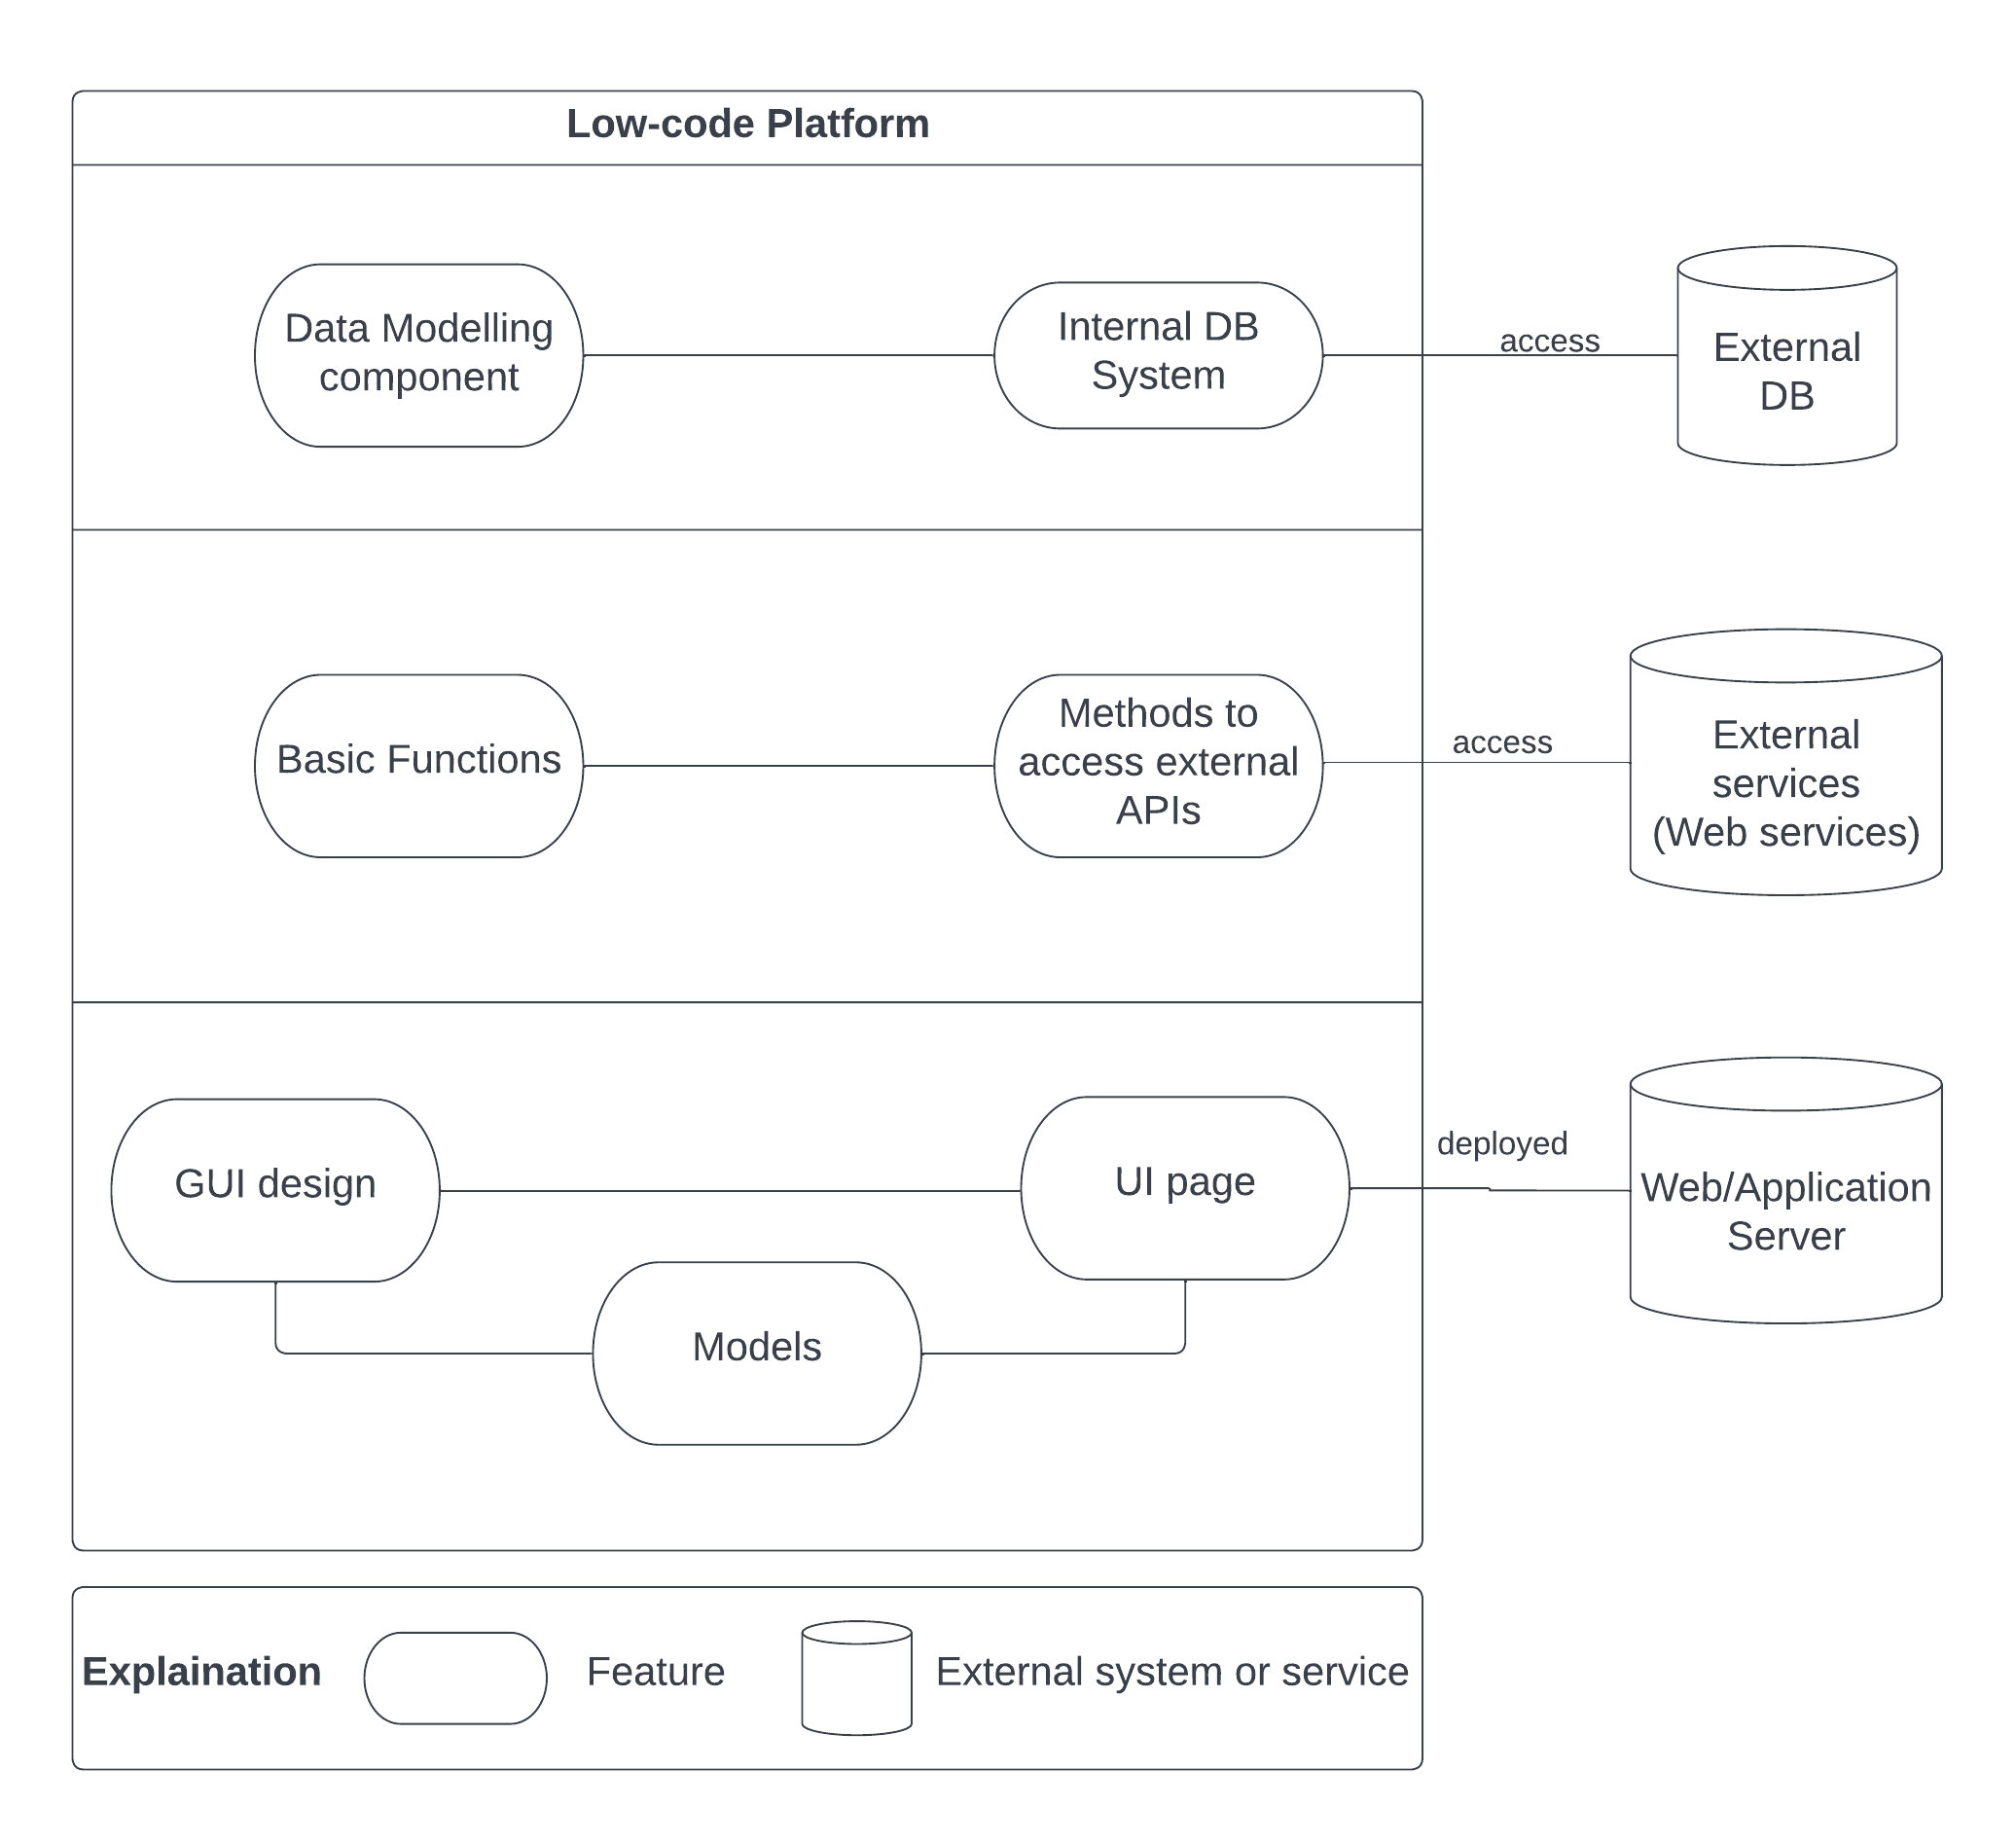
\includegraphics[width=0.73\textwidth]{LCDP-architecture.png}
  \caption[LCDP Architecture]{High-Level Architecture of Low Code Development Platform}
  \label{fig:background:architecture}
\end{figure}
\paragraph*{Functional Perspective:}
\ac{lcdp}s also offer basic functional specifications (see the second part of figure \ref{fig:background:architecture}). 
These typically include simple expression languages for decision rules and dialog-based methods for specifying program flow conditions. 
Each solution has a library of generic standard operations, such as mathematical functions. 
For example, \ac{lcdp}s will enable the use of traditional approaches such as web services and \ac{rest} services, and many modules provide support for a wide range of \ac{api}s from individual providers, such as Google \ac{api}s and social media \ac{api}s \cite{misc:lowcode:platforms}.
\paragraph*{Dynamic Perspective:}
The \ac{lcdp} also includes a \ac{gui} designer module (see the third part of \ref{fig:background:architecture}), allowing GUIs to be developed and integrated with other implementation elements.
The \ac{gui} designers module specifies pre-defined widgets, although the range varies. 
It is generally easy to link \ac{gui}s and \ac{ds}s in most of these platforms, as it is optional to manually implement the \ac{mvc} pattern.
In addition, many of these platforms offer specific support for adapting the \ac{gui}s to different target environments, such as desktop browsers, tablets, and smartphones \cite{paper:lowcode:cabot}.
Another common feature includes a component for defining roles and user rights, which is usually part of the platform's governing architecture and is deployed along with the custom application \cite{article:nocode:sahina}.\\\\
\textit{Main Steps Of \textbf{Low-Code} App Development} as per \cite{misc:lowcode:steps}:

\paragraph{Building:}
In this step, the platform allows you to alter the provided code and add hand-written custom code to specify more complex features as you create the app step-by-step using visual editors and drag-and-drop interfaces.
Modules, components, and chart-builders are already incorporated into low-code applications. 
Charts may be used to display data from modules, while modules are used to specify the type of data that will be stored in the app. 
Components and pages provide the type of user experience the app will have.
These platforms also have a provision for automating repetitive tasks in the app.

\paragraph{Testing:}
Testing a software application is an integral part of the development cycle.
However, the low-code development platform decreases the requirement for testing. 
Pre-build modules and components on low-code platforms are created with a certain level of application security. 
The developers of the low-code platform constantly monitor these modules, and they have previously gone through several unit tests.
But, in a low-code platform, testing can be performed in several ways \cite{misc:lowcode:testing}: \\\\
\textit{- Automated testing:} Some low-code platforms have built-in support for automated testing, which allows developers to create and run tests that validate the functionality of their applications.\\
\textit{- Manual testing:} Even with automated testing, it is necessary to perform manual testing to ensure that an application functions correctly. In a low-code platform, manual testing can be achieved by developers or by dedicated testers who are responsible for verifying the functionality of the application.\\
\textit{- \ac{uat}:} In some cases, it may be necessary to involve end users in the testing process. This can be done through user acceptance testing, which consists in having end users test the application and provide feedback on its functionality and usability.

Overall, testing in a \ac{lcdp} involves a combination of automated and manual testing, as well as performance and acceptance testing \cite{misc:lowcode:testing}, to ensure that the application is functioning correctly and meets the needs of end users.

\paragraph{Deploying:}
In this step, the application is deployed across apps and to the final users.
In \ac{lcdp}, the packages for installation, configurations, and application setup are included.
In terms of deployment, most of the considered solutions offer advanced support, although the specific forms vary. 
Some systems require the low-code platform environment to be installed on a web server to deploy individual applications. 
In contrast, others allow the developed solutions to be deployed as self-contained applications on various devices and machines.
This means that the \ac{lcdp} gives freedom to the users in deploying the applications for the customers with just one click. \\
\textit{Docker}\footnote{Website for Docker: \url{https://www.docker.com/}} is a widely used open software platform that allows applications to be deployed as containers. 
It supports libraries, system tools, code, and various runtimes, making it possible to build, test, deploy, and scale applications across multiple environments. 
In an \ac{lcdp}, docker can be used to securely deploy frameworks, services, and platforms in separate containers that communicate with each other using protocols such as \ac{mqtt}\footnote{Website for MQTT: The Standard for IoT Messaging \url{https://mqtt.org/}} and \ac{rest}\footnote{Website for REST / RESTful API: \url{https://www.redhat.com/en/topics/api/what-is-a-rest-api}}.
Additionally, a variety of options are provided for developers with little programming experience, those with coding expertise and seasoned programmers who wish to expand the functionality of the current design \cite{article:nocode:sahina}.

Overall, low-code/no-code development platforms are valuable for organizations looking to build and deploy custom applications quickly and efficiently that can help organizations of all sizes and industries bring their ideas to life.
\clearpage
%********************************** % Model-Based Software Engineering **************************************
\section{Model-Based Software Engineering}
\label{background:section:mbse}
\ac{mbse} refers to maintaining and developing software while reusing existing code.
Similarly, \ac{mdse} is the term used to cover various techniques for creating software using codified models.
At the same time, for creating models, the \ac{mof} has defined four levels separating the reality, models, meta-models, and meta-meta-models (as shown in figure \ref{fig:background:moflevels}).
\begin{figure}[htbp!]
  \centering    
  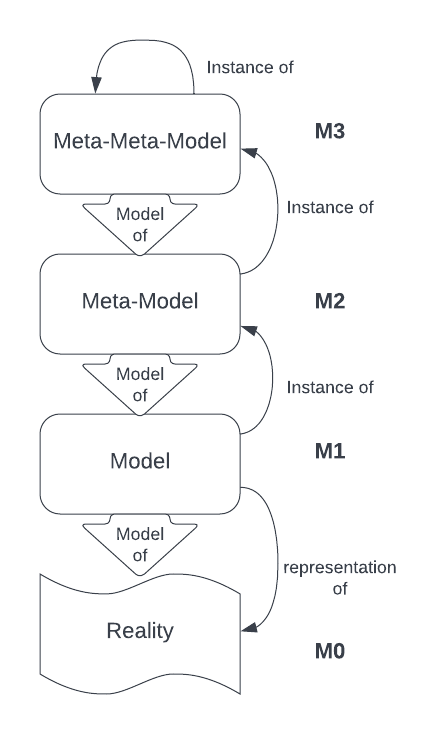
\includegraphics[width=0.5\textwidth]{mof-meta-modelling.png}
  \caption[MOF Levels]{Model Object Facility (MOF) levels}
  \label{fig:background:moflevels}
\end{figure}

\ac{mof} is a standard that defines a meta-model for modeling information. 
It provides a common framework for creating and using models representing a system or part of a technique used to analyze design or document the procedure.
\ac{mof} is part of the \ac{omg} \cite{misc:mbse:mof} standards and is used in several different contexts, including software engineering, business process modeling, and enterprise architecture. 
It is based on the \ac{uml}\footnote{Website for UML: \url{https://www.uml.org/}} standard notation for modeling software systems.
\ac{mof} defines a standard set of concepts and notations for creating and using models, which can represent different aspects of a system. 
This includes concepts such as classes, attributes, operations, and relationships, which describe the system's structure and behavior.

\paragraph{Meta-Models:} 
A meta-model is a model of a model or a simplified version of an actual model of a system of interest or a software application that formally represents the structure and behavior of a particular model type in a formal and standardized way.
Meta-models are often used in \ac{se} to describe the structure and behavior of \ac{dsl} or other modeling languages \cite{misc:metamodels:dsl}.
They can be used to understand how a model works or to improve the performance of a model by making it more efficient or accurate. 
Meta-models are often used in \ac{mdd}, focusing on creating and using high-level abstractions to design and implement software systems \cite{misc:metamodels:mdd}. 
Using meta-models, developers can create a high-level view of a system and then use that view to generate code automatically, which can help improve the development process's efficiency and reliability.
A model is usually defined as an abstraction of real-world entities, and a meta-model is another abstraction of the models. 
Similarly, metamodelling is analyzing and developing the rules, theories, and models helpful in constructing meta-models.

The \textbf{M0 layer} refers to the physical system or systems that are being modeled. 
It represents the real-world or the physical components, subsystems, and techniques that comprise the overall system being designed or analyzed. 
It is the foundation upon which the other layers of the \ac{mbse} models are built.

The \textbf{M1 layer}, built on top of the M0 layer, represents the functional requirements and system behavior.
The functional requirements include system inputs, outputs, and interfaces, and the system's behavior includes its response to different inputs and conditions.

The \textbf{M2 layer}, built on top of the M1 layer, represents the system's architecture and design. 
This layer describes how the system's components, subsystems, hardware, and software interact.
The M2 layer includes detailed specifications and design constraints such as interfaces, protocols, and data structures.

Finally, the \textbf{M3 layer} represents the system's implementation and verification. 
It includes the system's specific design details and implementation plans, including the detailed design of its components, selecting particular hardware and software, and testing and validation plans. 
This layer ensures that the system is built according to the specifications and design constraints defined in the M2 layer and meets the functional requirements and behavior described in the M1 layer.

After considering the information above, the meta-model can be further developed and refined. 
There are two approaches to designing a meta-model: \textit{Top-down and Bottom-up} \cite{misc:mbse:mof}. 
In the top-down method, we start with the overall process and then break it down into smaller steps. 
In the bottom-up approach, we begin with the individual steps and group them into more extensive procedures.
\textit{Top-down development} of a meta-model involves starting with a high-level representation of the structure and behavior of the models that the meta-model will describe (see figure \ref{fig:background:moflevels}). 
This high-level representation (M3 from figure \ref{fig:background:moflevels}) might include the overall design of the models (e.g., the types of elements and relationships that are allowed) and the rules and constraints that must be followed when creating and using the models.
Once the high-level structure of the meta-model has been defined, it can be further refined and expanded upon by adding lower-level details (M2 and M1 and M0 levels). 
They include the attributes and operations allowed for each element, how elements can be related, and the semantics of the relationships between elements.

\textit{Bottom-up development} of a meta-model involves starting with the specific elements and relationships that will be included in the meta-model and gradually building up to a higher level of abstraction. 
Once the lower-level details of the meta-model have been defined, they can be organized and grouped into higher-level concepts and structures, such as classes, packages, or packages of packages, to form the overall design of the meta-model \cite{misc:mbse:mof}.
\begin{figure}[htbp!]
  \centering    
  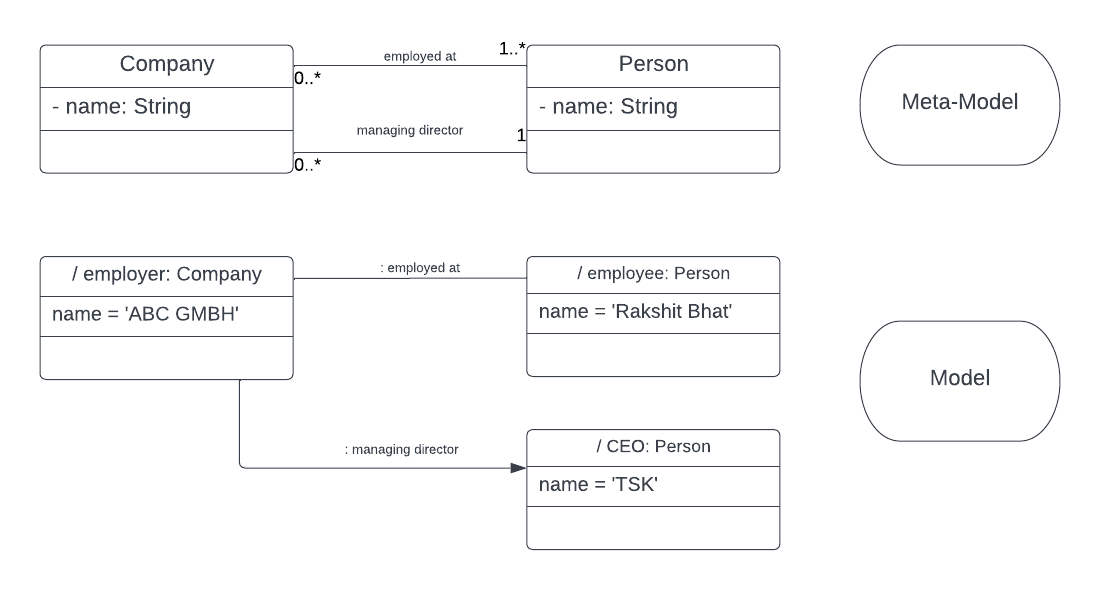
\includegraphics[width=0.9\textwidth]{meta-models.png}
  \caption[Meta Models]{Meta Models and Models}
  \label{fig:background:m1m2}
\end{figure}

\paragraph{Models:} 
As shown in figure \ref{fig:background:moflevels}, a \textit{Model} is a simplified representation of the real-world or reality.
Before any code is written, the model is a schematic that describes how the software system should function.
In software development, a model is a representation of a software system. 
It can be used to visualize the structure and behavior of a system or to analyze the system for potential issues or improvements. 
Models can take many forms, such as diagrams, graphs, or mathematical equations, and they can be created using various tools and techniques. 
Models are often used in \ac{mdd} \cite{misc:metamodels:mdd}, focusing on creating and using high-level abstractions to design and implement software systems. 
In this approach, models are used as the primary source of design and implementation information, and the code is generated from the models using a code generator \cite{article:mbse:bexiga}. 
By using models, developers can better understand a system and identify potential problems or areas for improvement before they start writing code.
From the example \ref{fig:background:m1m2}, we need to create models for every entity of reality (e.g., An employee and a CEO both are \textit{Person} in meta-model but are separate entities in models).
Using models, various adaptive model-driven \ac{ui} development systems are developed \cite{article:mbse:akiki} and the authors defined twenty properties challenges for the model-driven \ac{ui} and compared some tools that implement these properties.
Similarly, modeling is a process and method of building models for some purpose or related to some domain.
Therefore, models and modeling approaches are used to codify the \ac{ui}s in different companies. 

\ac{mbse} is a powerful approach to developing software that relies on using models to represent and analyze software systems. 
By using models to represent the various components and relationships within a software system, developers can more easily understand and analyze the system and make changes and updates more efficiently.
However, these models do not emphasize offering visual notations to aid non-developers in creating such interfaces. 
Therefore, for our research, we use a recent method \cite{article:mbse:bexiga}, which illustrates how to use low-code and model-driven approaches to close the gap between designers and developers.

\clearpage
%********************************** % Task-based Usability Testing **************************************
\section{Task-Based Usability Testing}
\label{background:section:task}
The main focus of usability testing is that seeing someone use an interface is the best approach to determine what functions well and what doesn't. 
It would help if you offered the participants some assignments to observe them. 
The word "task" is commonly used to describe these assignments.
Assigning tasks to the accurate number of participants can help determine the quality of the \ac{ui} and the problems faced by the users. 
Overall, the \ac{ui} design can be improved using the participants' feedback. 
Task-based usability testing is one way to determine the software's overall usability \cite{article:usability:doesburg} by measuring the percentage of the tasks the users complete.
These tasks need to be some scenarios, not just "\textit{do something}", because it sets the users a stage for \textit{why} they would perform the tasks. 
To get quality feedback from the participants, in \cite{misc:usability:tasks}, the authors provide \textit{three good practices} and task-writing tips for designing better task scenarios.

\paragraph{\textit{(1) Make the Task Realistic}:}
So, the participants should be able to execute the tasks which could be completed efficiently and with the freedom to make their own choices.
The participants will attempt to accomplish the assignment without genuinely interacting with the interface if you ask them to do something they wouldn't typically do. 
Therefore, it is necessary to create realistic tasks. \\\\
Task goal: The goal is to offer some movies that the user should watch. \\
\textbf{Bad task: } Watch a movie containing the actor `Mr. T' and actress `Ms. K'. \\
\textbf{Good Task: } Watch a movie with more than 6.5/10 ratings. \\
In the example, the participants should be free to compare movies based on their criteria. 

\paragraph{\textit{(2) Make the Task Actionable}:}
Here, the participants should be told what they need to do rather than how they would do it.
These types of tasks help us determine if the task isn't actionable enough.  
If the participants tell the moderator they cannot determine if they need to click on the link or if they are finding it hard to decide the next steps in a specific task, then it is a sign that the task needs to be more straightforward and actionable. \\\\
Task goal: The goal is to find a movie and show times. \\
\textbf{Bad Task: } You want to watch a movie Sunday afternoon. Go to the app and tell where you’d click next. \\
\textbf{Good Task: } Use the app to find a movie you'd be interested in watching on a sunday afternoon. \\

\paragraph{\textit{(3) Avoid Giving Clues and Describing the Steps}:}
There are frequent hints about how to use the interface or the software in step explanations.
These tasks must be more balanced with the users' behavior and give less valuable results.   
The participants should expose the navigation and some features on their own, giving accurate feedback about the interface.
But, at the same time, we should try to include the words used in the UIs as they help the users navigate smoothly and would not lead to some confusion. \\\\
Task goal: The goal is to change the user's movie preferences. \\
\textbf{Bad Task: } You want to change your movie preferences. Go to the website, sign in, and change your movie preferences. \\
\textbf{Good Task: } Change your movie preferences from `action' to `comedy'. \\\\
Therefore, it is crucial to create a realistic test environment during usability testing \cite{article:usability:doesburg}. 
It is also essential to provide the information required for the participant to complete the task without guiding them on specific actions. 
If the task scenario is unclear enough, the participant may ask for more information or confirm that they are on the correct path.

\begin{figure}[htbp!]
  \centering    
  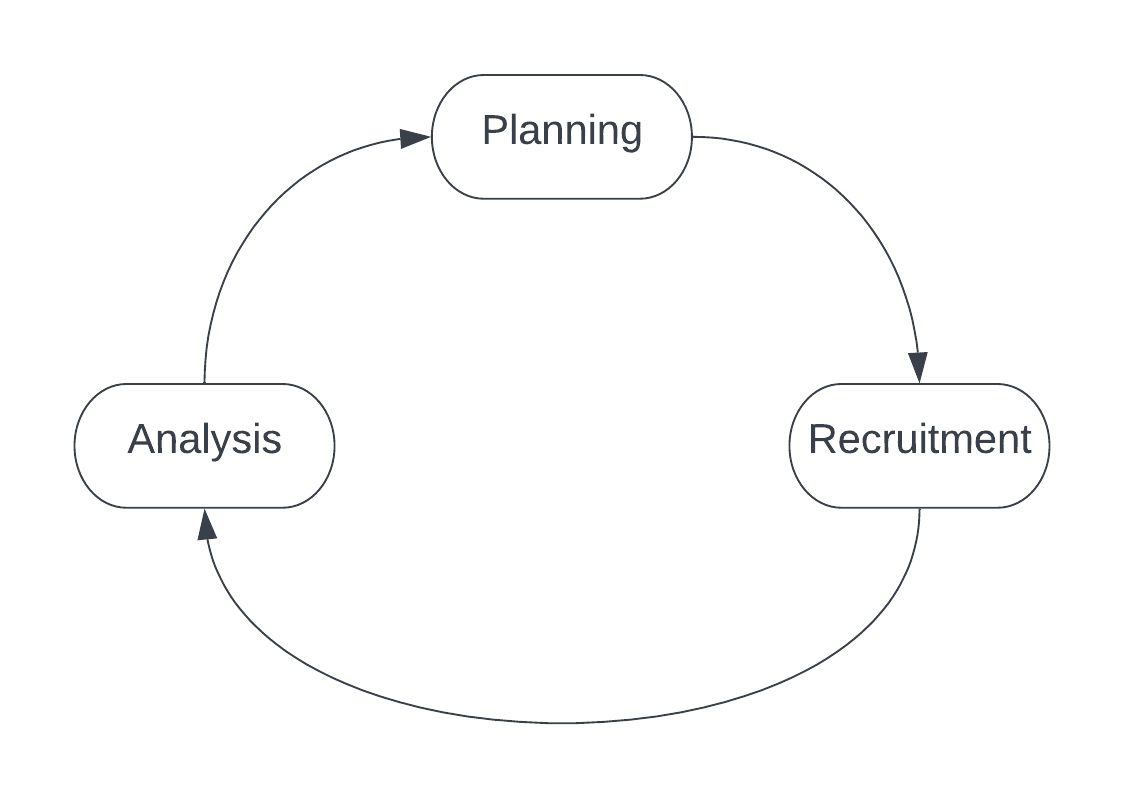
\includegraphics[width=0.6\textwidth]{task-based-cycle.png}
  \caption[Tasks Steps]{Task-Based Usability Testing Steps}
  \label{fig:background:taskssteps}
\end{figure}
The fundamental principle of usability testing is to have actual users attempt to carry out essential tasks or assignments on your software, websites, mobile applications, or gadgets.
For that, we divide task creation into three steps.
\paragraph{Planning:}
In usability testing, planning is an important step. 
In this step, we decide on a process that fits our research question, hypothesis, and metrics.  
It is beneficial if we use mixed-methods services for a task-based usability study.
The tasks and scenarios must be well-defined in the planning phase. At the same time, we can create pre-study and post-study questions. 
\paragraph{Recruitment:} 
In this step, the users are assigned to the task as it is essential to select the correct number of user group sizes.
There should be a proper way to interview the users before assigning them tasks so that the participants understand them correctly. 
The participants should also be able to ask questions or doubts while performing the honorarium tasks. 
\paragraph{Analysis:}
Task-based studies analyze metrics, issues, and insights in great depth.
For metrics, we calculate the task completion rates, task time, and task and test level perception questions.
The problems that the participants encounter while performing the tasks need to be reported automatically to the development teams by sending screenshots, quotes, etc. 
There should also be a section to analyze some insights about the software that has worked well for the users while performing the tasks.\\

Overall, task-based usability testing is a tool for evaluating the usability and effectiveness of software systems. 
By focusing on specific tasks that users need to complete, we can gather valuable insights into how well the system supports these tasks and identify areas where we could improve the \ac{ux}.
\clearpage

%********************************** % Experimentation **************************************
\section{UI Experimentation}
\label{background:section:experimentproduct}
In this section, we discuss the role that experimentation plays in the software development process and how designers can ``prototype with real data'' to improve the usability of the \ac{ui}.
Experimentation is a vital part of the design process for \ac{ui} products. 
It involves testing different design solutions and variations to see which performs best in terms of usability, aesthetics, and other desired characteristics \cite{article:controlled:experiements}. 
We can do this through various methods, such as usability testing, A/B testing, and rapid prototyping.
Experimentation allows designers to iterate and improve their designs by creating different \textit{`Software Variants'} and gathering data and feedback from real users.
It is an important part of creating user-centered designs that effectively meet the needs and expectations of the target audience \cite{article:experiments:lindgren}.
Experimentation helps product teams test out ideas early in the process with real-world consumers rather than settling on a single solution and executing it in the final phase \cite{misc:CE:miklos}.

\begin{figure}[htbp!]
  \centering    
  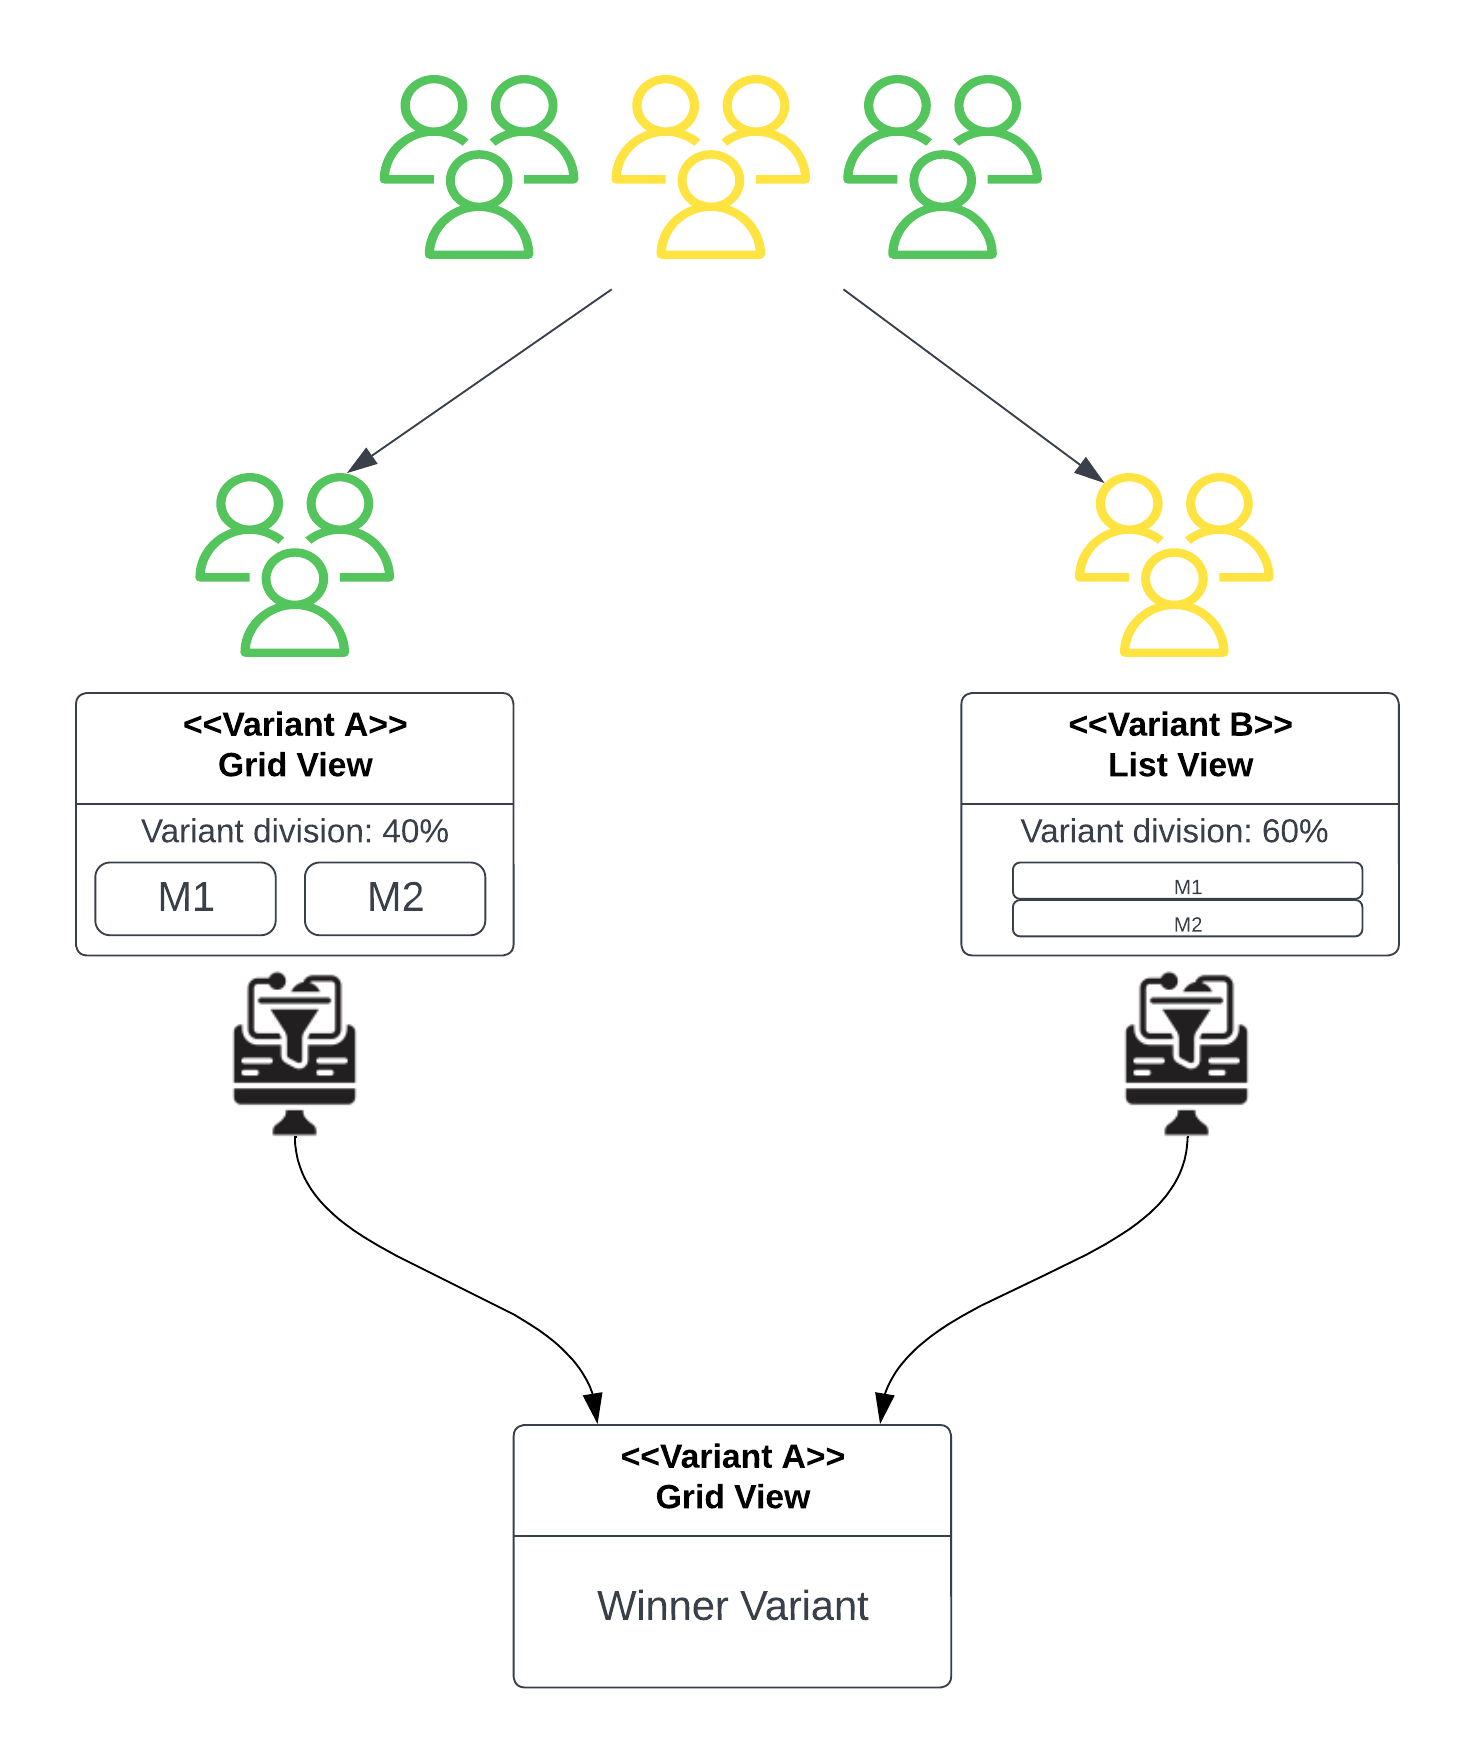
\includegraphics[width=0.5\textwidth]{variants.png}
  \caption[A/B Testing]{A/B Testing} 
  \label{fig:background:abtesting}
\end{figure}
For conducting experimentation, various steps like \textit{Users distribution}, \textit{\ac{ce}}, \textit{Variants distribution} exist.

\paragraph{User distribution:} To conduct a successful experiment, the size of the study, or the number of participants, must be considered first.
Statistics suggest that the more people you include in the investigation, the greater its statistical power, which impacts your level of confidence in your findings \cite{misc:experimentation:users}.
Then, the participants should be allocated into groups at random. 
There are several levels of treatment given to each group (e.g., some prerequisites to the participants before experimenting).
For assigning the subjects to groups, users are divided into a \textit{between-subjects design} vs a \textit{within-subjects design}.
In a between-subjects design, individuals receive only one of the possible levels of an experimental treatment whereas, in a within-subjects design, every individual receives each of the experimental treatments consecutively, and their responses to each treatment are measured.
In figure \ref{fig:background:abtesting}, a between-subject design is used where only one of the variants is assigned to the user.

\paragraph{Continuous Experimentation and Variants distribution:} 
\ac{ce} primarily aims to get users' feedback on the software product's evolution.
As per figure \ref{fig:background:abtesting}, \ac{ce} generally uses A/B testing in a primary case of comparing two variants, A and B, which are controlled and test variables in an experiment.
First, the users or the participants of the study are separated into groups and are assigned one of the two variants.
Since we have \texttt{GridView} and the \texttt{ListView}, one group of the users are assigned with List and one with Grid View (see figure \ref{fig:background:abtesting}).
Then both users would be given some tasks (see Section \ref{background:section:task}), and the analysis of these tasks gives the winner among the variants.
And in the end, developers make evidence-based decisions to direct the progress of their software by continuously measuring the results of multiple variants performed in an experimental context with actual users \cite{article:CE:ros}.
\ac{ce} is an extension to the introduction of continuous integration and deployment, and all are summarized as constant software engineering \cite{article:CE:fitzgerald}.
Additionally, \ac{ce} can help designers and developers stay up-to-date with the latest design trends and best practices. 
By regularly testing and iterating on the design, they can learn from the feedback they receive and incorporate new ideas and techniques into their design. 
This can help keep the product or service relevant and competitive \cite{article:controlled:experiements}.\\

Overall, \ac{ce} is a critical approach to take when developing \ac{ui}s for products and services. 
It allows designers and developers to gather valuable feedback and data and use it to improve their products' design and \ac{ux}.
\clearpage

\section{LEAN Development Process}
\label{background:section:lean}
LEAN development is a software development methodology that emphasizes continuous improvement and eliminating waste to deliver customer value as efficiently as possible. 
It is one method within Agile development \cite{misc:lean:tutorial}.
It is based on the principles of the LEAN manufacturing method, which was developed by \textit{Toyota} in the 1950s and aims to eliminate waste and maximize value in manufacturing processes \cite{misc:lean:toyota}.
LEAN development's primary objective was to reduce loss, minimize waste, and encourage sustainable production.
And therefore, as an \ac{mvp}, in LEAN development, the product has the essential elements necessary to launch successfully and does not have to include any additional components.

In software development, we can apply LEAN principles to various aspects of the development process, including requirements gathering, design, coding, testing, and deployment \cite{misc:lean:tutorial}.
The goal is to minimize waste and optimize the use of resources to deliver high-quality software products that meet the customer's needs.\footnotetext[8]{Website of the image: \url{https://www.agile-academy.com/en/agile-dictionary/lean-development/}}
\begin{figure}[htbp!]
  \centering    
  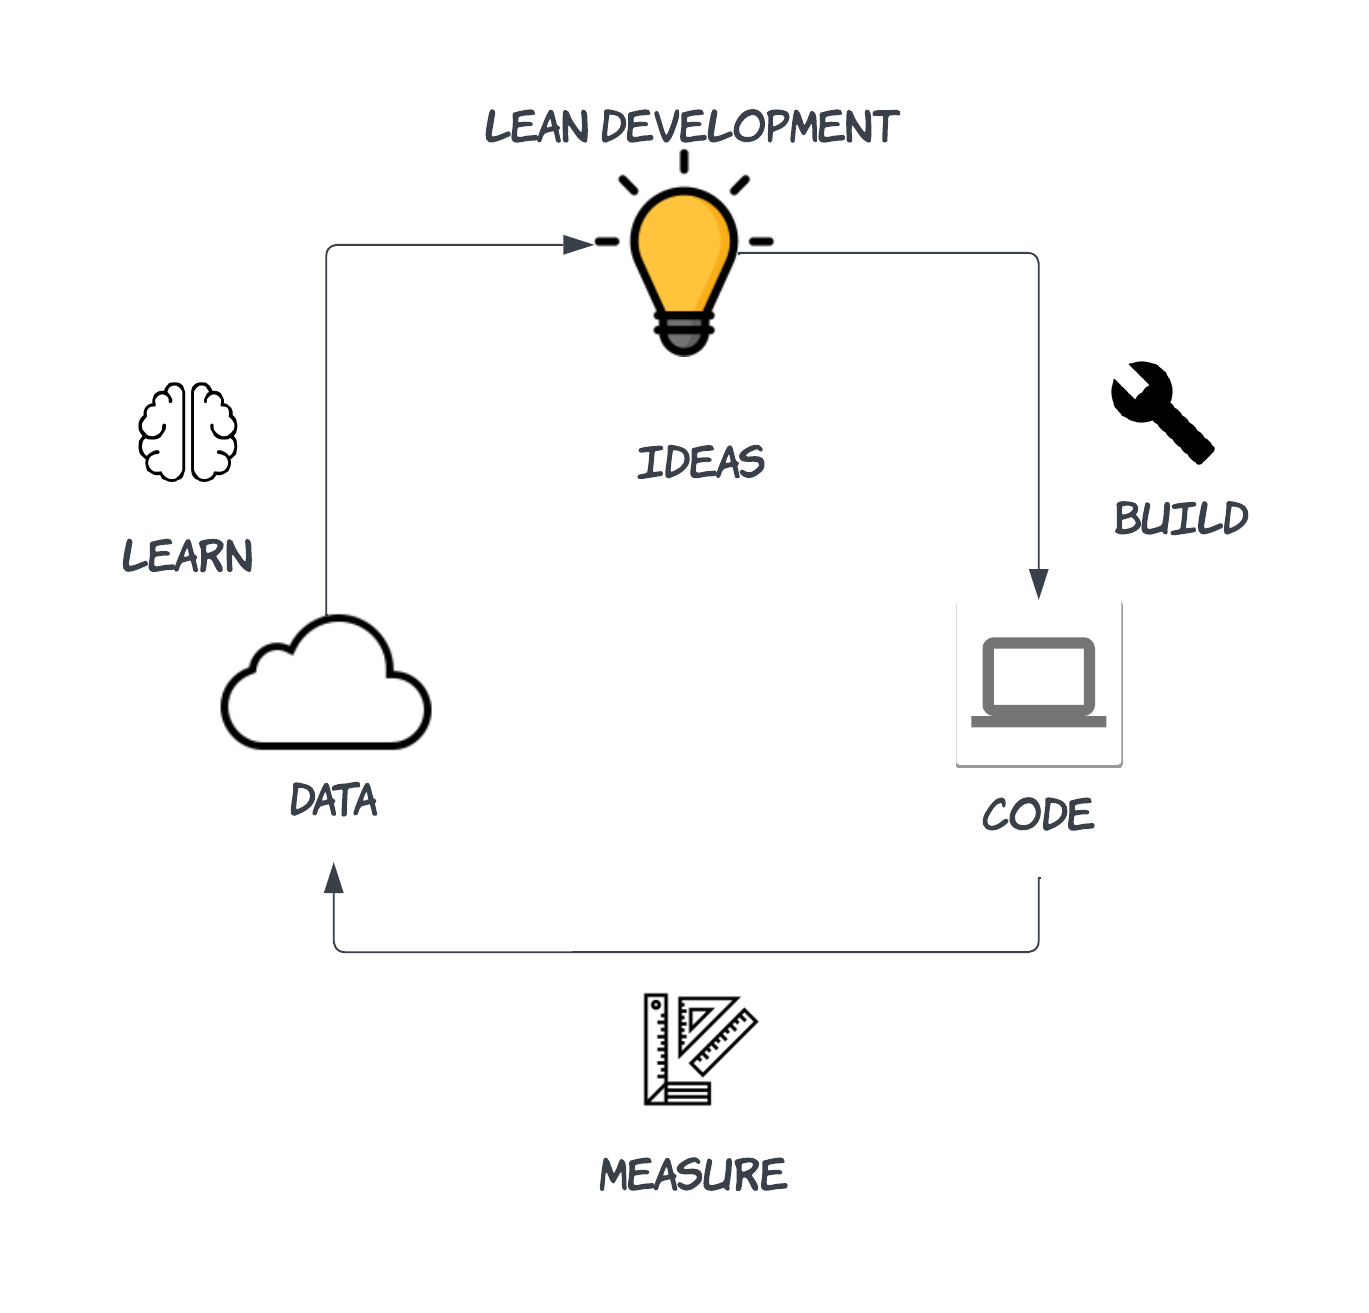
\includegraphics[width=0.7\textwidth]{LEAN.png}
  \caption[LEAN Development Cycle]{LEAN Development Cycle\footnotemark[8]}
  \label{fig:background:lean}
\end{figure}

\paragraph{LEAN Development Cycle:} 
The LEAN development cycle often includes three phases: \textit{Build, Measure, and Learn} (see figure \ref{fig:background:lean}). 
Steps like these are designed to help the development team continuously improve the product and development process.\\
\begin{itemize}
  \item[] \textbf{Build:} In the building phase of LEAN development, the development team works to build and deliver small increments of working software to the customer. This involves gathering requirements, designing, coding, testing, and deploying code \cite{misc:lean:tutorial}. The build phase's goal is to deliver customer requirements as quickly and efficiently as possible. To do this, the development team may follow model-driven development \cite{misc:lean:mdd}, continuous integration and delivery to ensure that the developed code meets the desired functionality and performance requirements.
  \item[] \textbf{Measure:} In the measurement phase of LEAN development, the development team collects data on the product's performance and the development process to identify areas for improvement \cite{misc:lean:tutorial}. It involves collecting data on customer usage and feedback, as well as data on the performance and efficiency of the development process. The measure phase aims to understand how the product is being used and its impact on the customer. It also identifies any bottlenecks or inefficiencies in the development process. The development team may use various tools and techniques, such as user testing, customer surveys, analytics data, and performance monitoring tools, to collect this data \cite{article:qqa:young, article:qq:helena}. They may also conduct regular reviews of the development process to identify improvement areas.
  \item[] \textbf{Learn:} In the learning phase of LEAN development, the development team uses the data collected in the measure phase to identify areas for improvement and make changes to the development process and the product \cite{misc:lean:tutorial}. It may involve making changes to the product roadmap, adjusting development practices, or implementing new tools or techniques \cite{article:lean:eric}. The goal of the learning phase is to improve the product continuously and the development process to deliver value to the customer more efficiently and effectively.
\end{itemize}
The final step in the cycle (see figure \ref{fig:background:lean}) would be to repeat the process, starting with identifying customer requirements and iterating through the \textit{Build}, \textit{Measure}, and \textit{Learn}\footnote{Website of LEAN cycle: \url{https://www.einstein1.net/build-measure-learn/}} phases again.
Thus, the development team can constantly improve the product and the development process to deliver value to the customer more efficiently and effectively. \\\\
As per \cite{misc:lean:tutorial}, there are some key practices in LEAN development.
These principles can be used to guide the discussion on which product development practices might be suitable for an organization, based on its specific circumstances.
\begin{itemize}
  \item[] \textbf{Continuous delivery:} Continuous delivery is the practice of regularly delivering small increments of working software to the customer rather than waiting until the end of the project to have a complete product. This allows the customer to see the project's progress and will enable them to give feedback and make changes as the project progresses. Continuous delivery helps to ensure that the software being developed meets the customer's needs and reduces the risk of delivering a product that does not meet their requirements \cite{article:lean:eric}. It also allows the development team to identify and fix problems early in the process, saving time and resources. To practice continuous delivery, the development team must have a process for automatically building, testing, and deploying code changes \cite{misc:lean:cicd}.
  \item[] \textbf{Continuous improvement:} Improving build quality in LEAN development refers to continuously improving the quality of the software being developed through effective coding practices, testing, and quality assurance processes \cite{misc:lean:cimp}. To improve the build quality, we can use \textit{Code reviews} \cite{misc:lean:tutorial}, i.e., conducting regular code review sessions to help identify problems early on and ensure that code meets standards for readability, maintainability, and performance. Similarly, implementing \textit{Quality Assurance} processes, such as testing, to catch and fix defects before they reach the customer can help improve the overall quality of the product.
  \item[] \textbf{LEAN planning:} It is a practice in LEAN development that focuses on maximizing value and minimizing waste in the software development process. It involves continuously prioritizing and reevaluating the work based on customer feedback to ensure that the team is first working on the most valuable features. As per \cite{misc:lean:planning}, LEAN planning aims to quickly identify and deliver the most valuable features to the customer while minimizing time and resources spent on non-critical tasks. This helps to ensure that the team is working on the right things and that the product meets the customer's needs. 
\end{itemize}
% \paragraph*{Benefits of Lean Development:} There are several benefits of LEAN development.Reduces project costs.
% Increases workflow efficiency and speed.
% Enables faster delivery of working products/software.
% Increases motivation of team members due to decision-making empowerment.
In this way, LEAN development can help organizations deliver high-quality products to customers more efficiently and effectively.
\clearpage
% \section{Foundation Summary}
% Finally, we explained how \ac{ui} prototyping allows for the rapid iteration and testing of design ideas before committing to development, improving the final product's overall usability and user experience.
% Then, we discussed how modeling allows for the simulation and analysis of complex systems and processes, enabling behavior prediction, identification of potential issues, and informed decision-making.
% Then, we also discussed how \ac{lcdp}s enable faster and more efficient software development by providing visual drag-and-drop interfaces, pre-built components, and automation, reducing the need for extensive coding knowledge.
% Then, we explained how Task-based usability testing evaluates a system's effectiveness by assigning users to complete specific tasks, providing valuable insights into the product's usability, and identifying areas for improvement.
% Finally, we explained how lean development could be used for continuous improvement, iterative product delivery, and collaborative teamwork to increase the efficiency of the product.

% In conclusion, the foundation chapter of the thesis is an integral part of the overall content. 
% It provides context and background information on the topic being discussed and helps the reader understand the purpose and significance of the thesis. 
% This section ensures the reader has the necessary information to understand and engage with the rest of the document completely.
% \clearpage

% \begin{landscape}

% \section{Landscape}
% I can cite Wall-E (see Fig.~\ref{fig:WallE}) and Minions in despicable me (Fig.~\ref{fig:Minnion}) or I can cite the whole figure as Fig.~\ref{fig:animations}


% \begin{figure}
%   \centering
%   \begin{subfigure}[b]{0.3\textwidth}
%     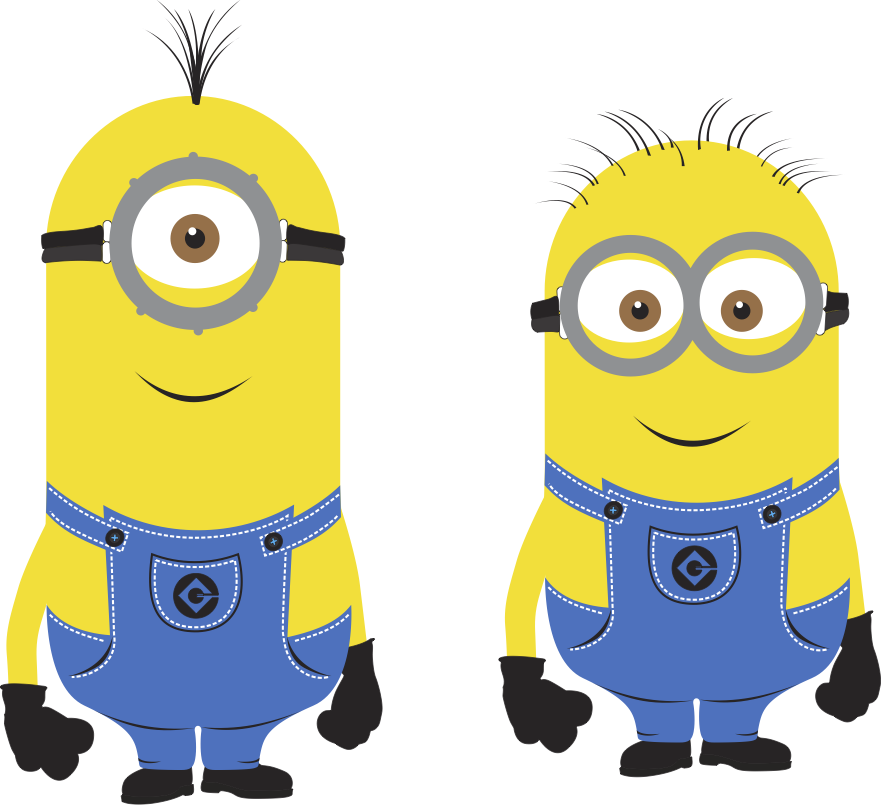
\includegraphics[width=\textwidth]{minion.png}
%     \caption{Tom and Jerry}
%     \label{fig:TomJerry}   
%   \end{subfigure}             
%   \begin{subfigure}[b]{0.3\textwidth}
%     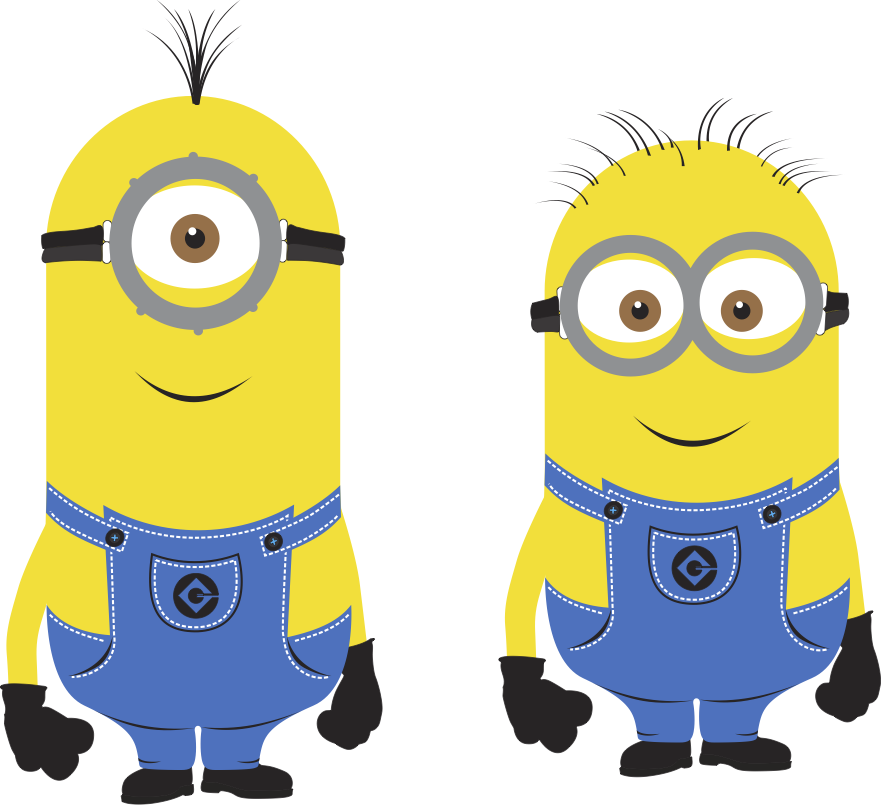
\includegraphics[width=\textwidth]{minion.png}
%     \caption{Wall-E}
%     \label{fig:WallE}
%   \end{subfigure}             
%   \begin{subfigure}[b]{0.3\textwidth}
%     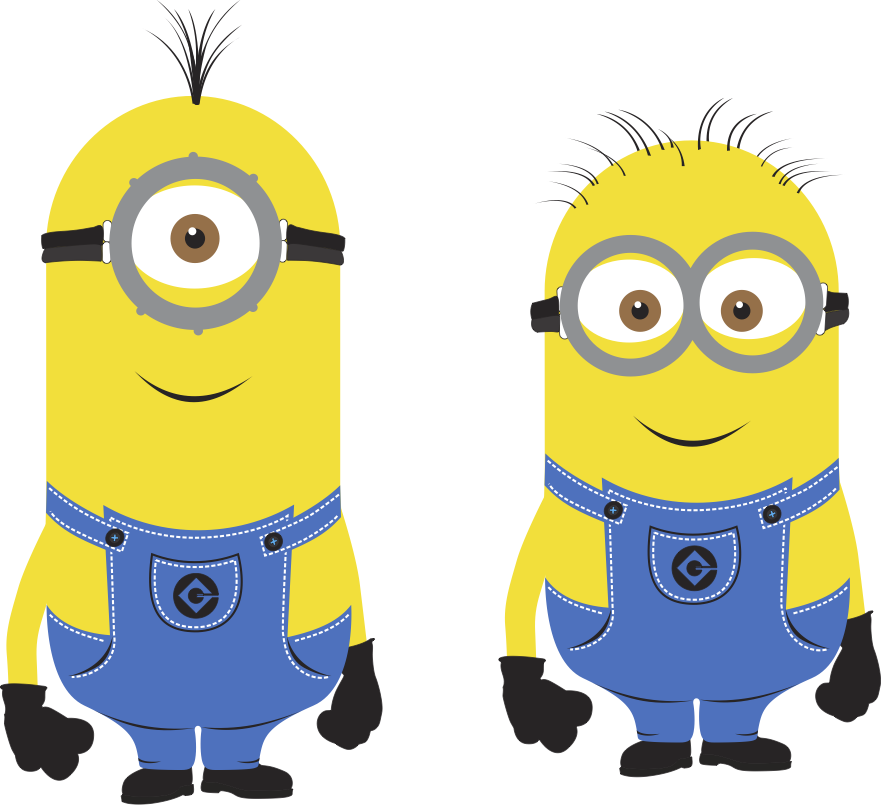
\includegraphics[width=\textwidth]{minion}
%     \caption{Minions}
%     \label{fig:Minnion}
%   \end{subfigure}
%   \caption{Best Animations}
%   \label{fig:animations}
% \end{figure}

% \end{landscape}
